\documentclass[border=4pt]{standalone}
% Shared preamble for every standalone pgfplots figure (compiled to PDF for the paper, SVG for the web).
\usepackage[T1]{fontenc}
\usepackage{newtxtext,newtxmath}
\usepackage{pgfplots,pgfplotstable}
\usepgfplotslibrary{groupplots,fillbetween}
\usetikzlibrary{arrows.meta,positioning,calc}
\pgfplotsset{compat=1.18}

% Palette (matches the matplotlib figures).
\definecolor{cJepa}{HTML}{1F4E79}
\definecolor{cFt}{HTML}{5B8FC9}
\definecolor{cRecon}{HTML}{B5562B}
\definecolor{cSup}{HTML}{3A7D44}
\definecolor{cGrey}{HTML}{6B6B6B}
\definecolor{cNominal}{HTML}{A8A8A8}
\definecolor{cPersist}{HTML}{C9B458}
\definecolor{cPi}{HTML}{8C6BB1}
\definecolor{cRandom}{HTML}{BDBDBD}
\definecolor{cMix}{HTML}{2A9D8F}
\definecolor{cHi}{HTML}{7A5195}
\definecolor{cHybrid}{HTML}{C0392B}

\pgfplotsset{
  every axis/.append style={
    font=\footnotesize, tick label style={font=\scriptsize}, label style={font=\footnotesize},
    title style={font=\footnotesize, yshift=-2pt}, legend style={font=\scriptsize, draw=none, fill=none},
    tick align=inside, minor tick num=1, axis line style={line width=0.5pt}, line width=0.9pt,
    legend cell align=left, every axis plot/.append style={line join=round},
  },
  panel/.style={width=7.6cm, height=5.2cm},
  colpanel/.style={width=8.0cm, height=5.6cm},
  every axis plot/.append style={mark options={solid, scale=0.7}},
  band/.style={draw=none, fill opacity=0.18, forget plot},
  rad/.style={ylabel={RMSE (rad\,s$^{-1}$)}},
}
\pgfplotstableset{col sep=comma}
\newcommand{\datadir}{../data}
% \bandplot{file}{x}{prefix}{colour}{legend}: mean line + min--max band over seeds.
\newcommand{\bandplot}[5]{%
  \addplot[name path=#3hi, draw=none, forget plot] table[x=#2, y=#3_hi] {#1};
  \addplot[name path=#3lo, draw=none, forget plot] table[x=#2, y=#3_lo] {#1};
  \addplot[#4, fill opacity=0.18, draw=none, forget plot] fill between[of=#3hi and #3lo];
  \addplot[#4, mark=*] table[x=#2, y=#3_m] {#1}; \addlegendentry{#5}}
% Same without a legend entry.
\newcommand{\bandplotnl}[4]{%
  \addplot[name path=#3hi, draw=none, forget plot] table[x=#2, y=#3_hi] {#1};
  \addplot[name path=#3lo, draw=none, forget plot] table[x=#2, y=#3_lo] {#1};
  \addplot[#4, fill opacity=0.18, draw=none, forget plot] fill between[of=#3hi and #3lo];
  \addplot[#4, mark=*, forget plot] table[x=#2, y=#3_m] {#1};}
\pgfplotsset{logticks/.style={ytick={1,2,5,10,20,50,100,200,500}, yticklabels={1,2,5,10,20,50,100,200,500}}}

\begin{document}
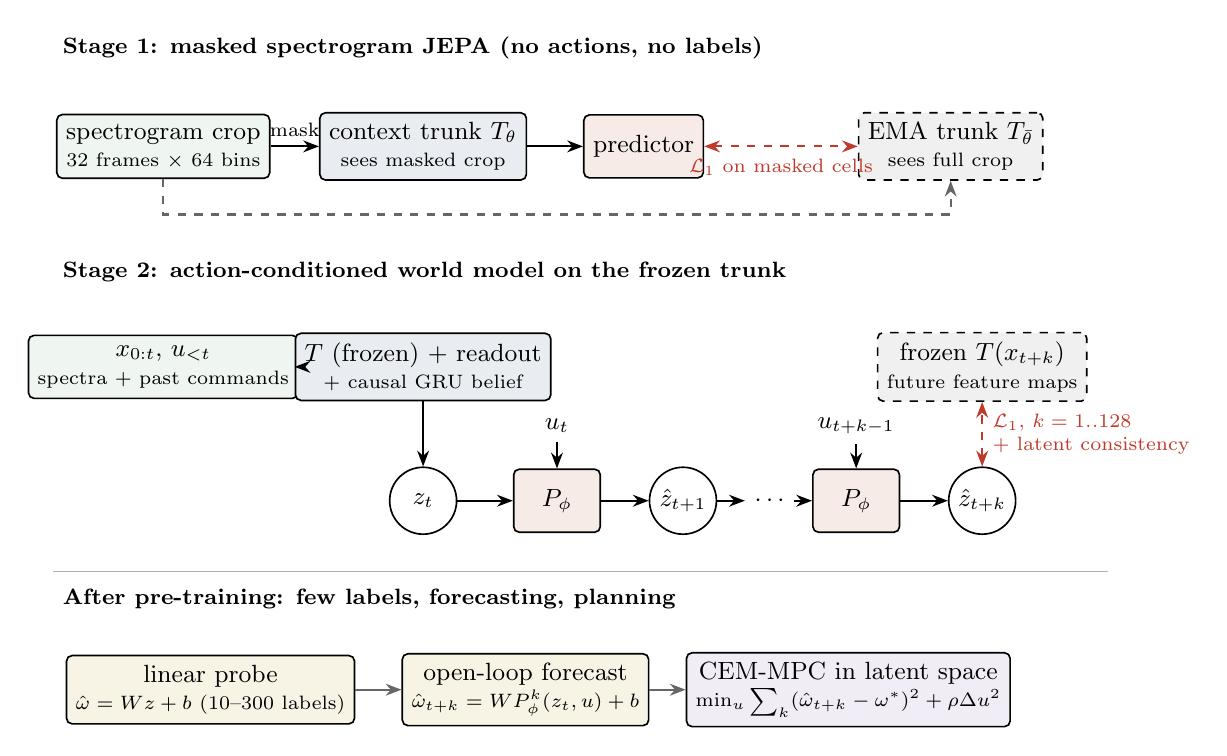
\begin{tikzpicture}[
  font=\small,
  box/.style={draw, rounded corners=2pt, minimum height=8mm, minimum width=18mm, align=center, fill=white, line width=0.6pt},
  enc/.style={box, fill=cJepa!10},
  tgt/.style={box, fill=black!6, dashed},
  pred/.style={box, fill=cRecon!12, minimum width=11mm},
  lat/.style={circle, draw, inner sep=0.5pt, minimum size=8.5mm, fill=white, line width=0.6pt},
  arr/.style={-{Stealth[length=2mm]}, line width=0.8pt},
  sg/.style={-{Stealth[length=2mm]}, line width=0.8pt, dashed, black!60},
]
% ---------------- stage 1
\node[font=\footnotesize\bfseries, anchor=west] at (-1.4,1.25) {Stage 1: masked spectrogram JEPA (no actions, no labels)};
\node[box, fill=cSup!8] (s1x) at (0,0) {spectrogram crop\\[-1pt]\scriptsize 32 frames $\times$ 64 bins};
\node[enc] (s1c) at (3.3,0) {context trunk $T_\theta$\\[-1pt]\scriptsize sees masked crop};
\node[pred] (s1p) at (6.1,0) {predictor};
\node[tgt] (s1t) at (10.0,0) {EMA trunk $T_{\bar\theta}$\\[-1pt]\scriptsize sees full crop};
\draw[arr] (s1x) -- node[above, font=\scriptsize] {mask} (s1c);
\draw[arr] (s1c) -- (s1p);
\draw[thick, dashed, cHybrid, <->, >={Stealth[length=2mm]}] (s1p) -- node[below, font=\scriptsize, text=cHybrid, yshift=-1pt] {$\mathcal L_1$ on masked cells} (s1t);
\draw[sg] (s1x.south) -- ++(0,-0.45) -| (s1t.south);
% ---------------- stage 2
\node[font=\footnotesize\bfseries, anchor=west] at (-1.4,-1.6) {Stage 2: action-conditioned world model on the frozen trunk};
\node[box, fill=cSup!8] (x0) at (0,-2.8) {$x_{0:t},\,u_{<t}$\\[-1pt]\scriptsize spectra + past commands};
\node[enc] (E) at (3.3,-2.8) {$T$ (frozen) + readout\\[-1pt]\scriptsize + causal GRU belief};
\node[lat] (zt) at (3.3,-4.5) {$z_t$};
\node[pred] (P1) at (5.0,-4.5) {$P_\phi$};
\node[lat] (z1) at (6.6,-4.5) {$\hat z_{t+1}$};
\node (dots) at (7.7,-4.5) {$\cdots$};
\node[pred] (Pk) at (8.8,-4.5) {$P_\phi$};
\node[lat] (zk) at (10.4,-4.5) {$\hat z_{t+k}$};
\node (u0) at (5.0,-3.55) {$u_t$};
\node (uk) at (8.8,-3.55) {$u_{t+k-1}$};
\node[tgt] (Y) at (10.4,-2.8) {frozen $T(x_{t+k})$\\[-1pt]\scriptsize future feature maps};
\draw[arr] (x0) -- (E); \draw[arr] (E) -- (zt);
\draw[arr] (zt) -- (P1); \draw[arr] (P1) -- (z1); \draw[arr] (z1) -- (dots); \draw[arr] (dots) -- (Pk); \draw[arr] (Pk) -- (zk);
\draw[arr] (u0) -- (P1); \draw[arr] (uk) -- (Pk);
\draw[thick, dashed, cHybrid, <->, >={Stealth[length=2mm]}] (zk) -- node[right, font=\scriptsize, text=cHybrid, align=left] {$\mathcal L_1$, $k=1..128$\\+ latent consistency} (Y);
% ---------------- use
\draw[black!30, line width=0.4pt] (-1.4,-5.4) -- (12.0,-5.4);
\node[font=\footnotesize\bfseries, anchor=west] at (-1.4,-5.75) {After pre-training: few labels, forecasting, planning};
\node[box, fill=cPersist!15] (probe) at (0.6,-6.9) {linear probe\\[-1pt]\scriptsize $\hat\omega=Wz+b$ (10--300 labels)};
\node[box, fill=cPersist!15] (roll) at (4.6,-6.9) {open-loop forecast\\[-1pt]\scriptsize $\hat\omega_{t+k}=W P_\phi^k(z_t,u)+b$};
\node[box, fill=cPi!12] (mpc) at (8.7,-6.9) {CEM-MPC in latent space\\[-1pt]\scriptsize $\min_u\sum_k(\hat\omega_{t+k}-\omega^\ast)^2+\rho\lVert\Delta u\rVert^2$};
\draw[arr, black!60] (probe) -- (roll); \draw[arr, black!60] (roll) -- (mpc);
\end{tikzpicture}
\end{document}
